
\chapter{Estabilidad de Lyapunov}

    Dada la siguiente representación de estado:

    \begin{equation} \label{eq:lyap1}
        \frac{dx(t)}{dt} = A x(t) + b u(t)
    \end{equation}

    con $x(0) = x_0  \in \mathbbm{R}^n$.

    \begin{definicion}
        El sistema representado por la ecuación ~\ref{eq:lyap1} es estable si para cada $\epsilon > 0$, existe un $\delta = \delta(\epsilon)$ tal que:

        \begin{equation*}
            ||x_0|| < \delta(\epsilon) \implies  ||x(t)||  < \epsilon \quad \forall t \ge 0
        \end{equation*}

        Si no es estable, decimos que es inestable.

        \begin{figure}
            \centering
            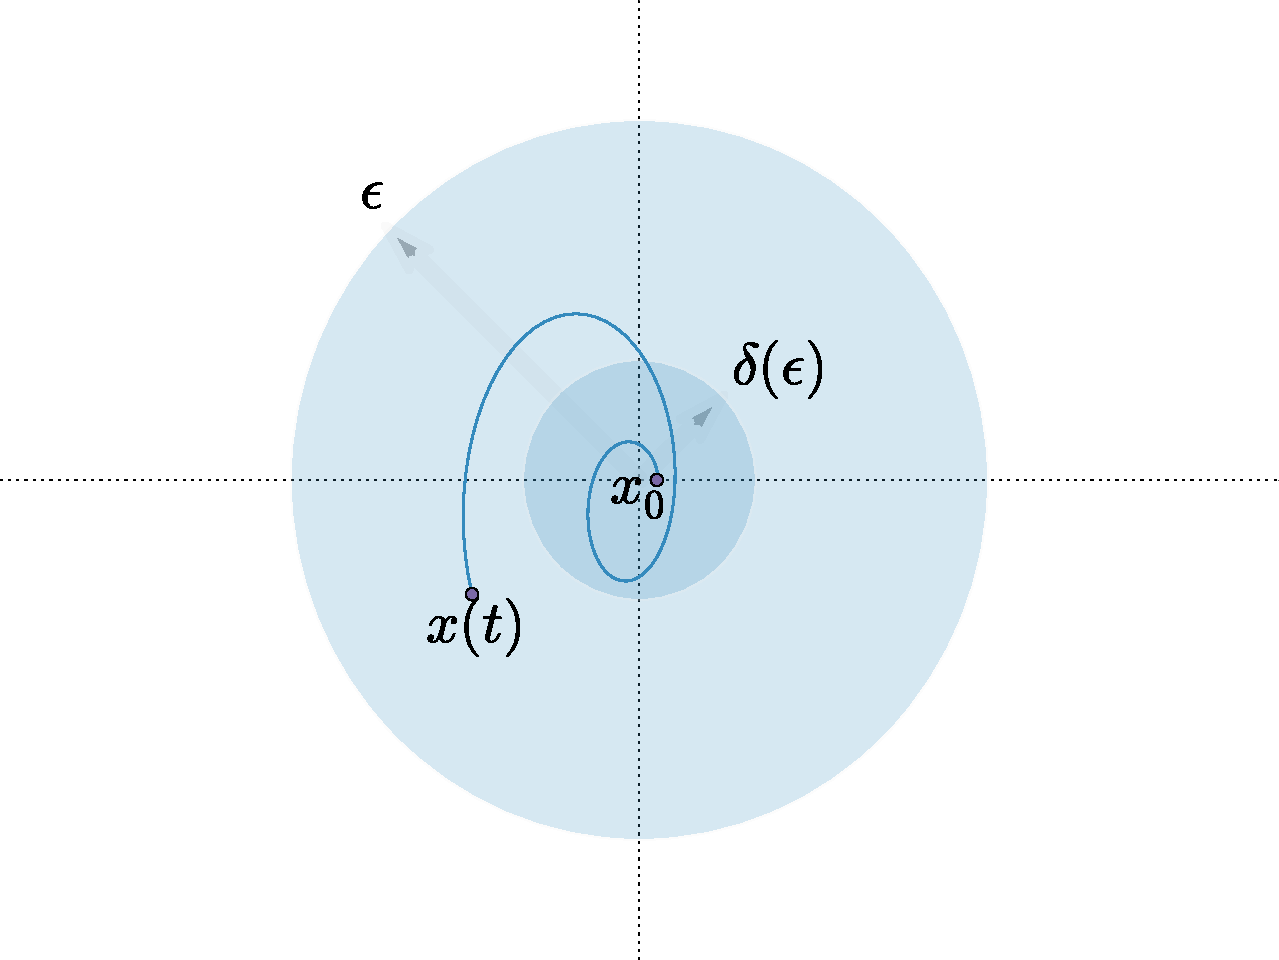
\includegraphics[width=0.7\textwidth]{./imagenes/trayectoriaacotada.pdf}
            \caption{\label{fig:trayectoriaestable}Trayectoria acotada por un limite $\epsilon$.}
        \end{figure}

        \missingfigure{Trayectoria acotada por un limite a traves del tiempo}

    \end{definicion}

    \begin{teorema} \label{te:lyap1}
        Una matriz $A$ es Hurwitz estable, es decir $\Re{\{ \lambda(A) \}} < 0$, si y solo si para cualquier matriz simetrica definida positiva dada, $Q$, existe una matriz  simetrica definida positiva, $P$, que satisface:

        \begin{equation}
            A^T P + P A = -Q
        \end{equation}

        \begin{nota}
            \tarea{Resumen de matrices Hermitianas de Introduction to Matrix Computations - G.W. Stewart Cap. 4 y 6}
            Una matriz $H \in \mathbbm{C}^{n\times n}$, se dice Hermitiana si su transpuesta conjugada es ella misma, $H^* = H$.
            Si $H \in \mathbbm{R}^{n \times n}$, se dice simétrica si su transpuesta es ella misma, $H^T = H$.

            De estas matrices, podemos notar ciertas propiedades:

            \begin{enumerate}
                \item Todos sus valores propios son reales.
                \item Cuando los valores propios de $H$ son todos positivos o negativos, se dice que $H$ es definida positiva o negativa, y se escribe $H > 0$ o $H < 0$ respectivamente.
                \item Cuando los valores propios de $H$ son todos no negativos o no positivos, se dice que $H$ es semidefinida positiva o semidefinida negativa y se escribe $H \ge 0$ o $H \le 0$ respectivamente.
                \item Desigualdad de Raleigh

                Dada $H$ Hermitiana:

                \begin{equation*}
                    \lambda_{min}(H) x^* x \le x^* H x \le \lambda_{max}(H) x^*x \quad \forall x \in \mathbbm{C}^n
                \end{equation*}

                Dada $H$ simétrica:

                \begin{equation*}
                    \lambda_{min}(H) x^T x \le x^T H x \le \lambda_{max}(H) x^T x \quad \forall x \in \mathbbm{C}^n
                \end{equation*}
                \item $H$ es semidefinida positiva, si y solo si, puede escribirse de la forma factorizada:

                \begin{equation*}
                    H = G^* G
                \end{equation*}

                para alguna matriz $G$, conocida como raiz cuadrada de $H$, tambien denotada por $H_{\sfrac{1}{2}}$, $\sqrt{H}$, $H^{\sfrac{1}{2}}$, por lo que la factorización queda como sigue:

                \begin{equation*}
                    H = H_{\sfrac{1}{2}}^* H_{\sfrac{1}{2}}
                \end{equation*}

                Cuando $H$ es definida positiva, $H_{\sfrac{1}{2}}$ es una matriz de rango pleno.
            \end{enumerate}
        \end{nota}
    \end{teorema}

    \begin{proof}
        \tarea{Resumen de estabilidad de Lyapunov de Linear Systems - Thomas Kailath Cap. 2.6}
        Sea la función de Lyapunov:

        \begin{equation} \label{eq:lyap2}
            V(x(t)) = x^T P x(t) \quad \forall t \ge 0
        \end{equation}

        con $P = P^T > 0$.

        Derivando a la ecuación ~\ref{eq:lyap2} con respecto del tiempo, a lo largo de las trayectorias solución de la ecuación ~\ref{eq:lyap1}, con $u = 0$, se tiene:

        \begin{eqnarray} \label{eq:lyap3}
            \frac{dV}{dt} & = & \frac{dx(t)}{dt}^T P x(t) + x^T(t) P \frac{dx(t)}{dt} \nonumber \\
            & = & x^T(t) A^T P x(t) + x^T(t) P A x(t) \nonumber \\
            & = & x^T(t) \left( A^T P + P A \right) x(t) \nonumber \\
            & = & -x^T(t) Q x(t)
        \end{eqnarray}

        Por otro lado, de la ecuación ~\ref{eq:lyap2} se tiene:

        \begin{equation*}
            \lambda_{min}(P) x^T(t) x(t) \le V(x(t)) \le \lambda_{max}(P) x^T(t) x(t)
        \end{equation*}

        por lo que:

        \begin{equation} \label{eq:lyap4}
            0 \le \frac{V(x(t))}{\lambda_{min}(P)} \le x^T(t) x(t) \le \frac{V(x(t))}{\lambda_{max}(P)}
        \end{equation}

        Entonces, de las ecuaciones ~\ref{eq:lyap3} y ~\ref{eq:lyap4} se obtiene:

        \begin{equation} \label{eq:lyap5}
            \frac{dV(x(t))}{dt} \le - \frac{\lambda_{min}(Q)}{\lambda_{max}(P)} V(x(t))
        \end{equation}

        De manera análoga

        \begin{equation*}
            \lambda_{min}(Q) x^T(t) x(t) \le x^T(t) Q x(t) \le \lambda_{max}(Q) x^T(t) x(t)
        \end{equation*}

        Si integramos la ecuación ~\ref{eq:lyap5} tendremos:

        \begin{equation*}
            \int_{0}^{t}\frac{dV(x(\tau))}{d\tau} d\tau \le - \frac{\lambda_{min}(Q)}{\lambda_{max}(P)} \int_{0}^{t} V(x(\tau)) d\tau
        \end{equation*}

        para lo cual necesitamos el lema de Bellman - Grönwall.\tarea{Feedback Systems - Input/Output Properties - Desoer, Vidyasagar Ap. E}

        \begin{nota}
            \begin{equation*}
                u(t) \le c + \int_0^t K(\tau) u(\tau) d\tau \implies u(t) \le c \exp{\left( \int_0^t K(\tau) d\tau \right)} \quad \forall t \ge 0
            \end{equation*}
        \end{nota}

        por lo tanto, podemos ver que:

        \begin{equation}
            V(x(t)) \le V(x(0)) - \frac{\lambda_{min}(Q)}{\lambda_{max}(P)} \int_0^t V(x(\tau)) d\tau
        \end{equation}

        y aplicando el lema de Bellman - Grönwall aqui:

        \begin{equation} \label{eq:lyap6}
            V(x(t)) \le V(x(0)) \exp{- \frac{\lambda_{min}(Q)}{\lambda_{max}(P)} t} \quad \forall t \ge 0
        \end{equation}

        de la ecuación ~\ref{eq:lyap4} y ~\ref{eq:lyap6}, obtenemos finalmente:

        \begin{equation*}
            0 \le x^T(t)x(t) \le \frac{\lambda_{max}(P)}{\lambda_{min}(P)} x^T(0)x(0) \exp{\left( - \frac{\lambda_{min}(Q)}{\lambda_{max}(P)} t \right)}
        \end{equation*}

        es decir:

        \begin{equation*}
            ||x(t)||^2 \le \frac{\lambda_{max}(P)}{\lambda_{min}(P)} ||x(0)||^2 \exp{\left( - \frac{\lambda_{min}(Q)}{\lambda_{max}(P)} t \right)}
        \end{equation*}

        \missingfigure{Función arbitraria acotada por una exponencial negativa.}

        Dado que $A$ es Hurwitz estable tenemos que $\Re{\lambda(A)} < 0$, sea la siguiente matriz definida positiva:

        \begin{equation*}
            P = \int_0^{\infty} \exp{(A^Tt)} Q \exp(At) dt
        \end{equation*}

        con $Q = Q^T > 0$. Entonces tendremos:

        \begin{eqnarray*}
            A^T P + P A & = & \int_0^{\infty} \left( A^T \exp{(A^T t)} Q \exp{(At)} + \exp{(A^T t)} Q \exp{(At)} A \right) dt \\
            & = & \int_0^{\infty} \frac{d}{dt} \left( \exp{(A^T t)} Q \exp{(At)} \right) dt \\
            & = & \left. \exp{(A^T t)} Q \exp{(At)} \right|_0^{\infty} \\
            & = & \lim_{t \to \infty} \exp{(A^T t)} Q \exp{(At)} - \exp{(A^T \cdot 0)} Q \exp{(A \cdot 0)} \\
            & = & 0 - Q = - Q
        \end{eqnarray*}
    \end{proof}

    \begin{lema}
        La ecuación matricial $A X = X B$, tiene unicamente la solución trivial, $X=0$, si y solo si, $A$ y $B$ no tienen valores propios en común, es decir:
        \begin{equation*}
            \sigma(A) \cap \sigma(B) \ne \emptyset
        \end{equation*}
    \end{lema}

    \begin{proof}
        \tarea{Buscar demostración en The Theory of Matrices - F.R. Gantmacher, Vol 1, Cap. 8}
    \end{proof}

    \begin{corolario} \label{co:lyap1}
        En el teorema~\ref{te:lyap1} se puede elegir a $Q$ como una matriz semidefinida positiva, $Q \ge 0$, bajo la condición inicial de que $x^T(t) Q x(t)$ no sea identicamente nula a lo largo de cualquier trayectoria no nula, solución de:

        \begin{equation*}
            \frac{d x(t)}{dt} = A x(t)
        \end{equation*}

        El requerimiento de este corolario se reduce a la condición de que el par $(Q_{\sfrac{1}{2}}, A)$ sea observable:

        \begin{equation*}
            Q \ge 0 \exists Q_{\sfrac{1}{2}} \text{ tal que } Q = Q_{\sfrac{1}{2}}^T Q_{\sfrac{1}{2}}
        \end{equation*}
    \end{corolario}

    \begin{corolario} \label{co:lyap2}
        Si $A$ es una matriz Hurwitz estable entonces la ecuación de Lyapunov, $A^T P + P A = -Q$, tiene una única solución para cada $Q$.
    \end{corolario}

    \begin{proof}
        Suponga que existen dos soluciones, $P_1$ y $P_2$, de la ecuación de Lyapunov, es decir:

        \begin{eqnarray*}
            A^T P_1 + P_1 A & = & -Q \\
            A^T P_2 + P_2 A & = & -Q
        \end{eqnarray*}

        lo cual implica:

        \begin{eqnarray*}
            A^T (P_2 - P_1) + (P_2 - P_1) A & = & 0 \\
            A^T (P_2 - P_1) - (P_2 - P_1) (-A) & = & 0 \\
        \end{eqnarray*}

        pero sabemos que el espectro de una matriz, no cambia debido a la transposición, $\sigma(A^T) = \sigma(A)$, y por otro lado tenemos que la matriz $A$ es Hurwitz estable, es decir $\Re{\left\{ \lambda(A)\right\}} < 0$, lo cual implica que:

        \begin{equation*}
            \Re{\left\{ \lambda(-A) \right\}} > 0
        \end{equation*}

        por lo que podemos concluir que:

        \begin{equation*}
            \sigma(A^T) \cap \sigma(-A) = \emptyset
        \end{equation*}

        por lo tanto, solo hay una solución y es la trivial.
    \end{proof}
